\section{Theorie}
\label{sec:Theorie}

\subsection{Dipole in Ionenkristallen}
Ionenkristallen bestehen aus einer regelmäßigen Anordnung von Anionen und Kationen.
Der im Versuch genutzt Kristall ist Kaliumbromid (KBr).
Dieses bildet ein kubisches Kristallsystem, indem Kalium nur Brom als Nachbaratom hat und umgekehrt.
Brom ist negativ geladen und bildet so die Anionen.
Kalium bildet im Gegenzug die Kation aufgrund der seiner geringeren Elektronegativität.
\\\\
Dies allein sorgt aber noch nicht für die Bildung von Dipolen im Kristall, dafür wird dem Kristall ein weiterer Stoff hinzugefügt.
Dieser Prozess wird Dotierung genannt, durch ihn können die Eigenschaften vom Kristall geändert werden.
In diesem Versuch wird dem Kaliumbromid mit einer Strontium Dotierung genutzt, dieses ist im Kristall doppelt positiv geladen.
Durch die doppelt positive Ladung verdrängt es ein Kationen also ein Kaliumion.
So ensteht ein Ladungsgefälle von dem Strontium zu der Leerstelle hin, was ein Dipolmoment zur Folge hat.
Verdeutlicht wird dies in \autoref{fig:dotierung}.
\begin{figure}
    \centering
    \caption{Die Entstehung von Dipolmomenten in Ionenkristallen durch Dotierung.}
    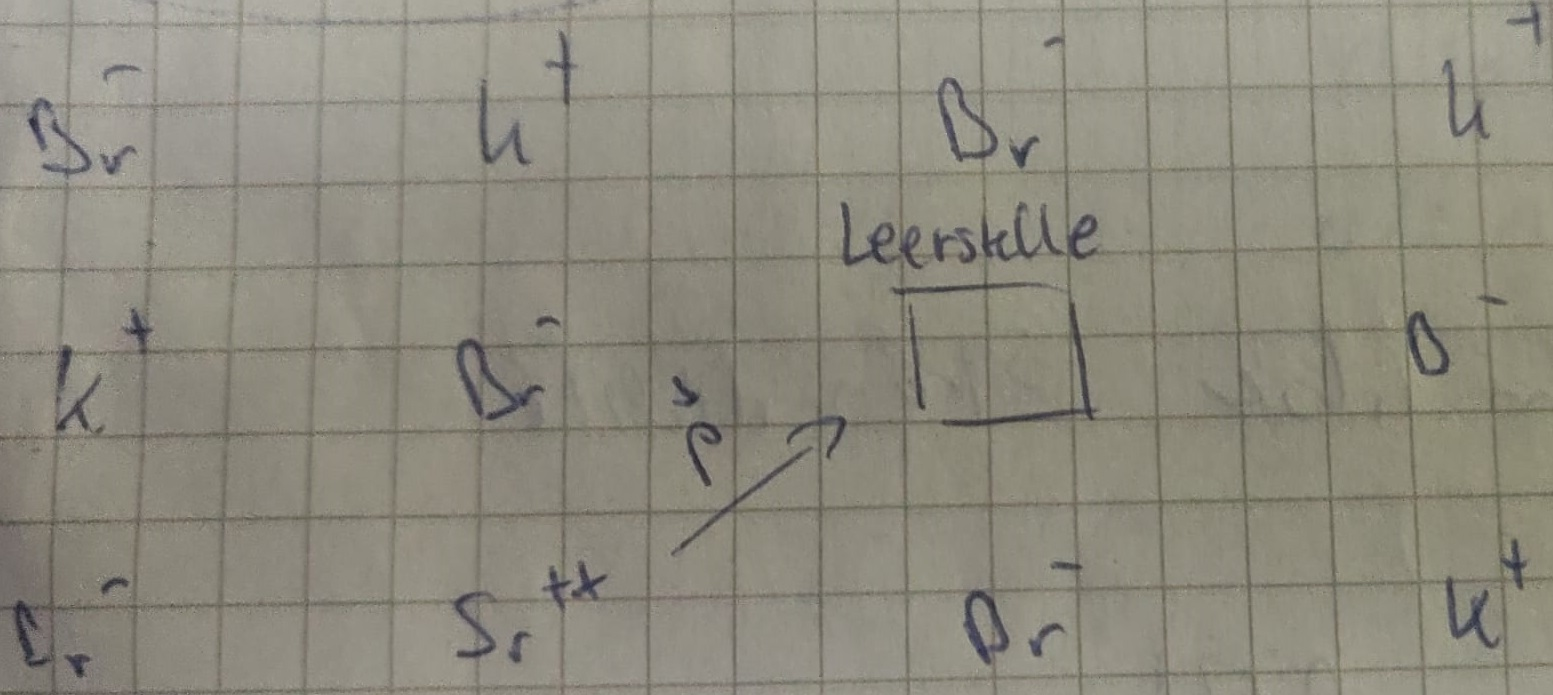
\includegraphics[width=\textwidth]{content/data/dotierung.jpeg}
    \label{fig:dotierung}
\end{figure}
Über Leerstellen Diffusion kann sich die Ausrichtung des Dipolmoments ändern.
Die Änderung kann zum Beispiel durch ein äußeres Feld hervorgerufen werden.
Ohne äußere Einflüsse ist die Ausrichtung der Dipole bei Raumtemperatur Boltzmann-Verteilt, sodass kein Gesamtdipolmoment vom Kristall ausgeht.
\\\\
Damit sich die Dipole wie erwähnt im E-Feld ausrichten können muss eine Aktivierungsenergie $W$ geleistet werden, die für die Leerstellendiffusion nötig ist.
Diese beeinflusst die Relaxationszeit der Dipole im Kristall.
Die Relaxationszeit im Kristall kann durch die Gleichung 
\begin{equation}
    \tau(T) = \tau_0 \exp( \frac{W}{k_\text{B} T})
    \label{eq:Relaxationszeit}
\end{equation}
bestimmt werden.
Wie aus der Gleichung zu entnehmen ist, hängt die Relaxationszeit auch von der Temperatur $T$ des Kristalls ab.
Zudem beschreibt $\tau_0$ die charakteristische Relaxationszeit und $k_\text{B}$ die Boltzmann-Konstante.

\subsection{Depolarisationsstrom}
Durch ein äußeres E-Feld richten sich die Dipole im Kristall aus, da sie der Richtung der Feldlinien folgen.
Hierdurch kommt es zur Polarisation.
Der Anteil der Dipole, der sich entlang der Feldlinien ausrichtet kann durch die Langevin Funktion
\begin{equation}
    y = L(x) = \coth(x)-\frac{1}{x} \qquad \text{mit} \qquad x=\frac{pE}{kT}
    \label{eq:Langevin}
\end{equation}
bestimmt werden.
Dies ist allerdings kein stabiler Zustand, denn die Dipole richten sich, sobald das E-Feld abgeschaltet wird wieder so aus, dass der Kristall kein Gesamtdipolmoment aufweist.
Durch diese Rückausrichtung der Dipole kann ein messbarer Strom induziert werden, welcher Depolarisationsstrom genannt wird.
Die Dipole richten sich dabei so lange aus, dass es wir erwähnt kein Gesamtdipolmoment mehr gibt und sie wieder Boltzmann-Verteilt sind.
Da sie aber nach Gleichung \eqref{eq:Relaxationszeit} für die Bewegung eine gewisse Aktivierungsenergie benötigen ist die wieder Ausrichtung bei sehr niedrigen Temperatur nur sehr langsam.


\subsection{Herleitungs des Depolarisationsstroms über den Polarisationsansatz}
Die Polarisation im Kristall ist durch Gleichung \eqref{eq:Langevin} gegeben.
Da für sehr hohe Temperatur der Zähler klein im Vergleich zum Nenner ist $pE << k_\text{B} T$ kann die Funktion durch eine Taylorentwicklung genähert werden.
Durch diese Näherung ergibt sich für die makroskopische Polarisation dann
\begin{equation}
    P = \frac{Np^2E}{3 k_\text{B}T} \, ,
    \label{eq:langevin2}
\end{equation}
welche sich aus der Summe aller mittleren Dipolmomente pro Volumen ergibt.
$N$ ist hier die Dichte der Dipole pro Volumen.
Die temperaturunabhängige Stromdichte $j(T)$ ist
\begin{equation}
    j(T) = P(T)p \frac{\symup{d}N}{\symup{d}t} \, ,
    \label{eq:stromdichte_unab}
\end{equation}
wobei $p$ das Dipolmoment und $P(T)$ der Anteil der ausgerichteten Dipole zur Temperatur $T$ angibt.
$\frac{\symup{d}N}{\symup{d}}t$ ist die Rate der Relation der Dipole.
Für die Rate der Relation der Dipole gilt
\begin{equation}
    \frac{\symup{d}N}{\symup{d}t} = \frac{-N}{\tau(T)}
\end{equation}
mit 
\begin{equation}
    N = N_\text{P} \exp{-\frac{1}{b} \int_{T_0}^{T} \frac{\symup{d}T'}{\tau{T'}}} \, .
\end{equation}
Dabei ist $N_\text{P}$ die Anzahl der ausgerichteten Dipole zum Beginn des Heizprozesses.
Durch einsetzen in Gleichung \eqref{eq:stromdichte_unab} ergibt sich nun der Depolarisationsstrom
\begin{equation}
    j(T) = \frac{p^2EN_\text{P}}{3 k_\text{B}T\tau_0} \exp{\frac{-W}{k_\text{B}T}} \exp{-\frac{1}{b} \int_{T_0}^{T} \frac{\symup{d}T'}{\tau{T'}}} \, .
\end{equation}
Diese kann zu 
\begin{equation}
    j(T) \approx  \frac{p^2EN_\text{P}}{3 k_\text{B}T\tau_0} \exp{\frac{-W}{k_\text{B}T}}
\end{equation}
Da bei kleinen Temperaturen und sehr großen Temperaturen kein Strom fließt.
Die Änderung der Polarisation ist gegeben durch
\begin{equation*}
    \frac{\symup{d}P}{\symup{d}t}=-\frac{P(t)}{\tau(T(t))} \, .
\end{equation*}
Hierbei beschreibt $P$ die Polarisation der Probe, welche dem Gesamtdipolmoment pro Volumeneinheit entspricht.
Die zeitliche Änderung der Polarisation indzuiert zudem de Strom
\begin{equation}
    I(t) = F\frac{\symup{d}P}{\symup{d}t} \, ,
\end{equation}
wobei $F$ den Probenquerschnitt angibt.
Durch Integration folgt 
\begin{equation}
    \tau(T) = \frac{ \int_{T}^{\infty} I(T')\symup{d}T'}{bI(T')}
\end{equation}
Dabei wird eine konstante Heizrate $b = \frac{\symup{d}T}{\symup{d}t}$ angenommen.
Durch gleichsetzen mit der Gleichung \eqref{eq:Relaxationszeit} ergibt sich
\begin{equation}
    \frac{W}{k_\text{b}T} = \frac{ \int_{T}^{\infty} I(T')\symup{d}T'}{\tau_0 b I(T')} \, ,
\end{equation}
woraus sich die Aktivierungsenergie $W$ ergibt.
Da bei der oberen Integrationskonstante $T=\infty$ kein Strom mehr induziert wird kann die maximale Relaxationszeit aus der Lage des ersten Maximums der Stromkurve bestimmt werden.
Durch Ableiten der Stromdichte \eqref{eq:stromdichte} folgt also
\begin{equation}
    \tau _\text{max}(T_\text{max}) = \frac{k_\text{b} T_\text{max} ^2}{bW}
\end{equation}
woraus wiederum durch einsetzen in Gleichung \eqref{eq:Relaxationszeit} die charakteristische Relaxationszeit $\tau_0$ bestimmten werden kann.


\subsection{Herleitung des Depolarisationsstroms über die Stromdichte}
Die Depolarisationsstromdichte setzt sich zusammen aus dem Anteil der ausgerichteten Dipole \eqref{eq:Langevin} bei einer Polarisationstemperatur $T_\text{p}$, dem Dipolmoment $p$ und der Relaxationsrate $\frac{\symup{d}N}{\symup{dt}}$ der Dipole pro Volumeneinheit
\begin{equation}
    j(T)=P(T)\, p \,\frac{\symup{d}N}{\symup{d}t} \stackrel{\eqref{eq:Langevin2}}{=} \frac{p^2 E}{3kT_p}\frac{\symup{d}N}{\symup{d}t} \, .
    \label{eq:stromdichte}
\end{equation}
Im Versuch wird eine konstanten Heizrate $b = \frac{\symup{d}T}{\symup{d}t}$ verwendet.
Mit dieser lässt sich die Relaxaktionsrate aus der Relaxationszeit \eqref{eq:Relaxationszeit} zu
\begin{align}
    \frac{\symup{d}N}{\symup{d}t} & = -\frac{N}{\tau(T)}\notag \\
    & = N_\text{p}\exp\left(-\frac{1}{b}\int_{T_0}^T \frac{\symup{d}T'}{\tau(T')}\right)
    \label{eq:Anzahl}
\end{align}
bestimmen.
Hierbei ist $N_\text{p}$ die Anzahl der ausgerichteten Dipole pro Volumeneinheit zum Zeitpunkt $t_0$ bei der Temperatur $T_0$.
Mit der Relaxationszeit \eqref{eq:Relaxationszeit} und der Anzahl der Dipole N \eqref{eq:Anzahl} ergibt sich für die Depolarisationsstromdichte \eqref{eq:stromdichte} der Ausdruck
\begin{equation}\label{eq:stromdichte2}
    j(T)= \frac{p^2E}{3kT_\text{p}}\frac{N_\text{p}}{\tau_0}\exp\left(-\frac{1}{b\tau_0}\int_{T_0}^T \exp\left(-\frac{W}{kT'}\symup{d}T'\right) \right)\exp\left(-\frac{W}{kT}\right)\, .
\end{equation}
Da die Temperatur zu Beginn des Depolarisationprozesses klein und somit $\exp(-\frac{W}{kT})\approx 0$ ist, ist stets
\begin{equation*}
    \int_{T_0}^T \exp\left(-\frac{W}{kT}\symup{d}T' \right) \approx 0\, ,
\end{equation*}
sodass für die Depolarisationsstromdichte im Anfangsbereich die Näherung
\begin{equation}
    j(T) \approx \frac{p^2 E}{3kT_\text{p}}\frac{N_\text{p}}{\tau_0}\exp\left(-\frac{W}{kT}\right)
    \label{eq:anlauf}
\end{equation}
gilt.
Daraus folgt, dass aus dem Verlauf des Depolarisationsstroms zu Beginn der Erwärmung die Aktivierungsenergie $W$, durch eine Ausgleichsrechung, bestimmt werden kann.
